% EchoScribe: single-file build. Needs only the figures/ folder next to it; the bibliography is
% embedded below (filecontents*) and written to refs.bib on the first run. The results macros come from
% eval/make_macros.py and are inlined in the preamble.
\begin{filecontents*}{refs.bib}
% EchoScribe — references (each entry checked against the publisher, PubMed, ACL Anthology or arXiv, Oct 2026)

% ── Documentation burden, formats, scribes ──
@article{weed1968,
  author  = {L. L. Weed},
  title   = {Medical records that guide and teach},
  journal = {N. Engl. J. Med.},
  volume  = {278},
  number  = {11},
  pages   = {593--600},
  year    = {1968}
}
@book{whitmore2017,
  author    = {J. Whitmore},
  title     = {Coaching for Performance: The Principles and Practice of Coaching and Leadership},
  edition   = {5th},
  publisher = {Nicholas Brealey},
  address   = {London, U.K.},
  year      = {2017}
}
@article{sinsky2016,
  author  = {C. Sinsky and others},
  title   = {Allocation of physician time in ambulatory practice: A time and motion study in 4 specialties},
  journal = {Ann. Intern. Med.},
  volume  = {165},
  number  = {11},
  pages   = {753--760},
  year    = {2016}
}
@article{tierney2024,
  author  = {A. A. Tierney and others},
  title   = {Ambient artificial intelligence scribes to alleviate the burden of clinical documentation},
  journal = {NEJM Catal. Innov. Care Deliv.},
  volume  = {5},
  number  = {3},
  year    = {2024}
}
@article{lukac2025,
  author  = {P. J. Lukac and W. Turner and S. Vangala and A. T. Chin and J. Khalili and Y. T. Shih and C. Sarkisian and E. M. Cheng and J. N. Mafi},
  title   = {Ambient {AI} scribes in clinical practice: A randomized trial},
  journal = {NEJM AI},
  volume  = {2},
  number  = {12},
  year    = {2025},
  doi     = {10.1056/AIoa2501000}
}
@article{wang2025scribe,
  author  = {H. Wang and others},
  title   = {An evaluation framework for ambient digital scribing tools in clinical applications},
  journal = {npj Digit. Med.},
  volume  = {8},
  pages   = {358},
  year    = {2025},
  doi     = {10.1038/s41746-025-01622-1}
}
@article{xu2025laos,
  author  = {Y. Xu and H. Jia and M. Wang and J. Feng and others},
  title   = {Enhancing clinical documentation with voice processing and large language models: A study on the {LAOS} system},
  journal = {npj Digit. Med.},
  volume  = {8},
  pages   = {798},
  year    = {2025},
  doi     = {10.1038/s41746-025-02170-4}
}

% ── Note generation and summarisation ──
@inproceedings{benabacha2023eacl,
  author    = {A. {Ben Abacha} and W.-W. Yim and G. Adams and N. Snider and M. Yetisgen},
  title     = {An empirical study of clinical note generation from doctor-patient encounters},
  booktitle = {Proc. EACL},
  pages     = {2291--2302},
  year      = {2023}
}
@inproceedings{benabacha2023mediqa,
  author    = {A. {Ben Abacha} and W.-W. Yim and G. Adams and N. Snider and M. Yetisgen},
  title     = {Overview of the {MEDIQA-Chat} 2023 shared tasks on the summarization \& generation of doctor-patient conversations},
  booktitle = {Proc. 5th Clinical Natural Language Processing Workshop},
  pages     = {503--513},
  year      = {2023},
  doi       = {10.18653/v1/2023.clinicalnlp-1.52}
}
@article{yim2023aci,
  author  = {W.-W. Yim and Y. Fu and A. {Ben Abacha} and N. Snider and T. Lin and M. Yetisgen},
  title   = {{ACI-BENCH}: A novel ambient clinical intelligence dataset for benchmarking automatic visit note generation},
  journal = {Sci. Data},
  volume  = {10},
  pages   = {586},
  year    = {2023}
}
@article{vanveen2024,
  author  = {D. {Van Veen} and others},
  title   = {Adapted large language models can outperform medical experts in clinical text summarization},
  journal = {Nat. Med.},
  volume  = {30},
  number  = {4},
  pages   = {1134--1142},
  year    = {2024},
  doi     = {10.1038/s41591-024-02855-5}
}
@inproceedings{wang2025acl,
  author    = {H. Wang and others},
  title     = {Towards adapting open-source large language models for expert-level clinical note generation},
  booktitle = {Findings Assoc. Comput. Linguistics: ACL 2025},
  pages     = {12084--12117},
  year      = {2025},
  doi       = {10.18653/v1/2025.findings-acl.626}
}
@article{adhikary2024,
  author  = {P. K. Adhikary and others},
  title   = {Exploring the efficacy of large language models in summarizing mental health counseling sessions: Benchmark study},
  journal = {JMIR Ment. Health},
  volume  = {11},
  pages   = {e57306},
  year    = {2024}
}

% ── Hallucination, grounding, verification ──
@article{ji2023survey,
  author  = {Z. Ji and others},
  title   = {Survey of hallucination in natural language generation},
  journal = {ACM Comput. Surv.},
  volume  = {55},
  number  = {12},
  year    = {2023}
}
@article{asgari2025,
  author  = {E. Asgari and others},
  title   = {A framework to assess clinical safety and hallucination rates of {LLMs} for medical text summarisation},
  journal = {npj Digit. Med.},
  volume  = {8},
  pages   = {274},
  year    = {2025},
  doi     = {10.1038/s41746-025-01670-7}
}
@inproceedings{gao2023alce,
  author    = {T. Gao and H. Yen and J. Yu and D. Chen},
  title     = {Enabling large language models to generate text with citations},
  booktitle = {Proc. EMNLP},
  pages     = {6465--6488},
  year      = {2023}
}
@inproceedings{min2023factscore,
  author    = {S. Min and others},
  title     = {{FActScore}: Fine-grained atomic evaluation of factual precision in long form text generation},
  booktitle = {Proc. EMNLP},
  pages     = {12076--12100},
  year      = {2023}
}
@inproceedings{manakul2023selfcheck,
  author    = {P. Manakul and A. Liusie and M. J. F. Gales},
  title     = {{SelfCheckGPT}: Zero-resource black-box hallucination detection for generative large language models},
  booktitle = {Proc. EMNLP},
  pages     = {9004--9017},
  year      = {2023}
}
@inproceedings{dhuliawala2024cove,
  author    = {S. Dhuliawala and others},
  title     = {Chain-of-verification reduces hallucination in large language models},
  booktitle = {Findings Assoc. Comput. Linguistics: ACL 2024},
  pages     = {3563--3578},
  year      = {2024}
}

% ── Diarization, enhancement, recognition ──
@article{park2022review,
  author  = {T. J. Park and others},
  title   = {A review of speaker diarization: Recent advances with deep learning},
  journal = {Comput. Speech Lang.},
  volume  = {72},
  year    = {2022}
}
@inproceedings{desplanques2020ecapa,
  author    = {B. Desplanques and J. Thienpondt and K. Demuynck},
  title     = {{ECAPA-TDNN}: Emphasized channel attention, propagation and aggregation in {TDNN} based speaker verification},
  booktitle = {Proc. Interspeech},
  pages     = {3830--3834},
  year      = {2020}
}
@article{vonluxburg2007,
  author  = {U. {von Luxburg}},
  title   = {A tutorial on spectral clustering},
  journal = {Stat. Comput.},
  volume  = {17},
  number  = {4},
  pages   = {395--416},
  year    = {2007}
}
@inproceedings{plaquet2023powerset,
  author    = {A. Plaquet and H. Bredin},
  title     = {Powerset multi-class cross entropy loss for neural speaker diarization},
  booktitle = {Proc. Interspeech},
  pages     = {3222--3226},
  year      = {2023},
  doi       = {10.21437/Interspeech.2023-205}
}
@inproceedings{park2025sortformer,
  author    = {T. Park and others},
  title     = {Sortformer: A novel approach for permutation-resolved speaker supervision in speech-to-text systems},
  booktitle = {Proc. ICML},
  series    = {PMLR},
  volume    = {267},
  year      = {2025}
}
@inproceedings{wang2024diarizationlm,
  author    = {Q. Wang and others},
  title     = {{DiarizationLM}: Speaker diarization post-processing with large language models},
  booktitle = {Proc. Interspeech},
  pages     = {3754--3758},
  year      = {2024},
  doi       = {10.21437/Interspeech.2024-209}
}
@inproceedings{bain2023whisperx,
  author    = {M. Bain and J. Huh and T. Han and A. Zisserman},
  title     = {{WhisperX}: Time-accurate speech transcription of long-form audio},
  booktitle = {Proc. Interspeech},
  year      = {2023}
}
@misc{zolensky2025,
  author       = {A. Zolensky and K. J. Jang and J. Sabin and others},
  title        = {Speaker role identification in clinical conversations},
  howpublished = {medRxiv preprint},
  year         = {2025},
  doi          = {10.1101/2025.08.14.25332837}
}
@inproceedings{subakan2021sepformer,
  author    = {C. Subakan and M. Ravanelli and S. Cornell and M. Bronzi and J. Zhong},
  title     = {Attention is all you need in speech separation},
  booktitle = {Proc. IEEE ICASSP},
  pages     = {21--25},
  year      = {2021}
}
@misc{ravanelli2021speechbrain,
  author       = {M. Ravanelli and others},
  title        = {{SpeechBrain}: A general-purpose speech toolkit},
  howpublished = {arXiv:2106.04624},
  year         = {2021}
}
@inproceedings{wichern2019wham,
  author    = {G. Wichern and others},
  title     = {{WHAM!}: Extending speech separation to noisy environments},
  booktitle = {Proc. Interspeech},
  year      = {2019}
}
@article{dubey2024dns,
  author  = {H. Dubey and others},
  title   = {{ICASSP} 2023 Deep Noise Suppression Challenge},
  journal = {IEEE Open J. Signal Process.},
  volume  = {5},
  pages   = {725--737},
  year    = {2024}
}
@inproceedings{iwamoto2022,
  author    = {K. Iwamoto and T. Ochiai and M. Delcroix and others},
  title     = {How bad are artifacts?: Analyzing the impact of speech enhancement errors on {ASR}},
  booktitle = {Proc. Interspeech},
  year      = {2022}
}
@inproceedings{radford2023whisper,
  author    = {A. Radford and others},
  title     = {Robust speech recognition via large-scale weak supervision},
  booktitle = {Proc. ICML},
  year      = {2023}
}
@inproceedings{panayotov2015librispeech,
  author    = {V. Panayotov and G. Chen and D. Povey and S. Khudanpur},
  title     = {Librispeech: An {ASR} corpus based on public domain audio books},
  booktitle = {Proc. IEEE ICASSP},
  pages     = {5206--5210},
  year      = {2015}
}
@inproceedings{watanabe2020chime6,
  author    = {S. Watanabe and others},
  title     = {{CHiME-6} challenge: Tackling multispeaker speech recognition for unsegmented recordings},
  booktitle = {Proc. 6th Int. Workshop on Speech Processing in Everyday Environments (CHiME)},
  year      = {2020}
}
@inproceedings{bredin2017metrics,
  author    = {H. Bredin},
  title     = {pyannote.metrics: A toolkit for reproducible evaluation, diagnostic, and error analysis of speaker diarization systems},
  booktitle = {Proc. Interspeech},
  year      = {2017}
}

% ── LLMs, routing, metrics ──
@misc{gemini2023,
  author       = {{Gemini Team, Google}},
  title        = {Gemini: A family of highly capable multimodal models},
  howpublished = {arXiv:2312.11805},
  year         = {2023}
}
@misc{openai2025gptoss,
  author       = {{OpenAI}},
  title        = {gpt-oss-120b \& gpt-oss-20b model card},
  howpublished = {arXiv:2508.10925},
  year         = {2025}
}
@misc{ong2024routellm,
  author       = {I. Ong and others},
  title        = {{RouteLLM}: Learning to route {LLMs} with preference data},
  howpublished = {arXiv:2406.18665},
  year         = {2024}
}
@article{chen2024frugalgpt,
  author  = {L. Chen and M. Zaharia and J. Zou},
  title   = {{FrugalGPT}: How to use large language models while reducing cost and improving performance},
  journal = {Trans. Mach. Learn. Res.},
  year    = {2024}
}
@misc{omniroute2026,
  author       = {{OmniRoute contributors}},
  title        = {{OmniRoute}: Open-source {AI} gateway with combo routing and provider cooldowns, v3.8.52},
  howpublished = {\url{https://github.com/diegosouzapw/OmniRoute}},
  note         = {MIT License},
  year         = {2026}
}
@inproceedings{lin2004rouge,
  author    = {C.-Y. Lin},
  title     = {{ROUGE}: A package for automatic evaluation of summaries},
  booktitle = {Text Summarization Branches Out (ACL Workshop)},
  pages     = {74--81},
  year      = {2004}
}
@inproceedings{zhang2020bertscore,
  author    = {T. Zhang and V. Kishore and F. Wu and K. Q. Weinberger and Y. Artzi},
  title     = {{BERTScore}: Evaluating text generation with {BERT}},
  booktitle = {Proc. ICLR},
  year      = {2020}
}
@techreport{jain1984fairness,
  author      = {R. Jain and D.-M. Chiu and W. R. Hawe},
  title       = {A quantitative measure of fairness and discrimination for resource allocation in shared computer systems},
  institution = {Digital Equipment Corporation},
  number      = {DEC-TR-301},
  year        = {1984}
}

% ── Risk screening ──
@article{posner2011cssrs,
  author  = {K. Posner and others},
  title   = {The {Columbia-Suicide Severity Rating Scale}: Initial validity and internal consistency findings from three multisite studies with adolescents and adults},
  journal = {Am. J. Psychiatry},
  volume  = {168},
  number  = {12},
  pages   = {1266--1277},
  year    = {2011}
}
@article{kroenke2001phq9,
  author  = {K. Kroenke and R. L. Spitzer and J. B. W. Williams},
  title   = {The {PHQ-9}: Validity of a brief depression severity measure},
  journal = {J. Gen. Intern. Med.},
  volume  = {16},
  number  = {9},
  pages   = {606--613},
  year    = {2001}
}
@article{levkovich2023,
  author  = {I. Levkovich and Z. Elyoseph},
  title   = {Suicide risk assessments through the eyes of {ChatGPT-3.5} versus {ChatGPT-4}: Vignette study},
  journal = {JMIR Ment. Health},
  volume  = {10},
  pages   = {e51232},
  year    = {2023},
  doi     = {10.2196/51232}
}
@inproceedings{guo2017calibration,
  author    = {C. Guo and G. Pleiss and Y. Sun and K. Q. Weinberger},
  title     = {On calibration of modern neural networks},
  booktitle = {Proc. ICML},
  pages     = {1321--1330},
  year      = {2017}
}

@inproceedings{bredin2023pyannote,
  author    = {Herv{\'e} Bredin},
  title     = {pyannote.audio 2.1 speaker diarization pipeline: principle, benchmark, and recipe},
  booktitle = {Proc. Interspeech},
  pages     = {1983--1987},
  year      = {2023},
  doi       = {10.21437/Interspeech.2023-105}
}

@inproceedings{korfiatis2022primock57,
  author    = {Papadopoulos Korfiatis, Alex and Moramarco, Francesco and Sarac, Radmila and Savkov, Aleksandar},
  title     = {{PriMock57}: A dataset of primary care mock consultations},
  booktitle = {Proc. 60th Annual Meeting of the Association for Computational Linguistics (Volume 2: Short Papers)},
  address   = {Dublin, Ireland},
  pages     = {588--598},
  year      = {2022},
  doi       = {10.18653/v1/2022.acl-short.65}
}

@inproceedings{wu2022annomi,
  author    = {Wu, Zixiu and Balloccu, Simone and Kumar, Vivek and Helaoui, Rim and Reiter, Ehud and Reforgiato Recupero, Diego and Riboni, Daniele},
  title     = {{Anno-MI}: A dataset of expert-annotated counselling dialogues},
  booktitle = {Proc. IEEE ICASSP},
  pages     = {6177--6181},
  year      = {2022},
  doi       = {10.1109/ICASSP43922.2022.9746035}
}
\end{filecontents*}
\documentclass[conference]{IEEEtran}
\IEEEoverridecommandlockouts
\usepackage{iftex}
\ifPDFTeX
  \usepackage[utf8]{inputenc}
\fi
% T1 Times under pdfLaTeX (Overleaf) and XeTeX (Tectonic) alike, as IEEEtran expects
\usepackage[T1]{fontenc}
\usepackage{cite}
\usepackage{amsmath,amssymb}
\usepackage{graphicx}
\usepackage{booktabs}
\usepackage{xcolor}
\usepackage{url}
\usepackage{tikz}
\usetikzlibrary{positioning,fit,arrows.meta,shapes.geometric,calc}
\usepackage[hidelinks]{hyperref}

% Results, generated by eval/make_macros.py from eval/results/*; it also defines the switches
% \ifrecheck and \ifmentoring, which are true only when those experiments are complete.
% Generated by eval/make_macros.py — do not edit by hand
\newif\ifrecheck
\newif\ifmentoring
\newcommand{\ResAblBert}{49.8}
\newcommand{\ResAblHeldAgree}{87.7\%}
\newcommand{\ResAblHeldNotes}{11}
\newcommand{\ResAblHeldPartial}{9.6\%}
\newcommand{\ResAblHeldSentences}{260}
\newcommand{\ResAblHeldSupported}{87.3\%}
\newcommand{\ResAblHeldSupportedCi}{82.7--90.8}
\newcommand{\ResAblHeldUnsupported}{3.1\%}
\newcommand{\ResAblNotes}{40}
\newcommand{\ResAblRepNotesUnsupported}{0}
\newcommand{\ResAblRepPartial}{1.5\%}
\newcommand{\ResAblRepSupported}{98.5\%}
\newcommand{\ResAblRepUnsupported}{0.0\%}
\newcommand{\ResAblRepairFlagged}{60}
\newcommand{\ResAblRepairRemoved}{12}
\newcommand{\ResAblRepairRewritten}{44}
\newcommand{\ResAblRougeL}{49.4}
\newcommand{\ResAblRougeOne}{53.0}
\newcommand{\ResAblRougeTwo}{21.8}
\newcommand{\ResAblSentences}{905}
\newcommand{\ResAblVerNotesUnsupported}{17}
\newcommand{\ResAblVerPartial}{3.0\%}
\newcommand{\ResAblVerSupported}{93.4\%}
\newcommand{\ResAblVerUnsupported}{3.6\%}
\newcommand{\ResAnnoCited}{96.4\%}
\newcommand{\ResAnnoJudgeGeminiN}{39}
\newcommand{\ResAnnoJudgeGroqN}{1}
\newcommand{\ResAnnoNotesN}{40}
\newcommand{\ResAnnoPartial}{13.3\%}
\newcommand{\ResAnnoRoleCombined}{40}
\newcommand{\ResAnnoRoleHardCombined}{17}
\newcommand{\ResAnnoRoleHardLlm}{17}
\newcommand{\ResAnnoRoleHardN}{17}
\newcommand{\ResAnnoRoleHardStats}{16}
\newcommand{\ResAnnoRoleLlm}{40}
\newcommand{\ResAnnoRoleN}{40}
\newcommand{\ResAnnoRoleStats}{38}
\newcommand{\ResAnnoSentences}{549}
\newcommand{\ResAnnoSupported}{80.3\%}
\newcommand{\ResAnnoUnsupported}{6.4\%}
\newcommand{\ResAudioCpGemAudioClean}{17.8}
\newcommand{\ResAudioCpGemAudioFive}{37.1}
\newcommand{\ResAudioCpGemAudioZero}{59.3}
\newcommand{\ResAudioCpPyaPropClean}{21.4}
\newcommand{\ResAudioCpPyaPropFive}{47.1}
\newcommand{\ResAudioCpPyaPropZero}{68.8}
\newcommand{\ResAudioCpPyaWordsClean}{2.6}
\newcommand{\ResAudioCpPyaWordsFive}{19.7}
\newcommand{\ResAudioCpPyaWordsZero}{53.2}
\newcommand{\ResAudioCpSbEnhClean}{43.4}
\newcommand{\ResAudioCpSbEnhFive}{48.8}
\newcommand{\ResAudioCpSbEnhZero}{77.9}
\newcommand{\ResAudioCpSbRawClean}{34.1}
\newcommand{\ResAudioCpSbRawFive}{49.7}
\newcommand{\ResAudioCpSbRawZero}{65.2}
\newcommand{\ResAudioCpSbWordsClean}{21.0}
\newcommand{\ResAudioCpSbWordsFive}{27.1}
\newcommand{\ResAudioCpSbWordsZero}{46.9}
\newcommand{\ResAudioCpTextClean}{38.4}
\newcommand{\ResAudioCpTextFive}{34.9}
\newcommand{\ResAudioCpTextZero}{62.0}
\newcommand{\ResAudioDerPyaClean}{9.3}
\newcommand{\ResAudioDerPyaFive}{12.9}
\newcommand{\ResAudioDerPyaZero}{22.6}
\newcommand{\ResAudioDerSbEnhClean}{27.3}
\newcommand{\ResAudioDerSbEnhFive}{19.4}
\newcommand{\ResAudioDerSbEnhZero}{26.3}
\newcommand{\ResAudioDerSbRawClean}{23.1}
\newcommand{\ResAudioDerSbRawFive}{25.1}
\newcommand{\ResAudioDerSbRawZero}{24.9}
\newcommand{\ResAudioWerGemEnhClean}{4.0}
\newcommand{\ResAudioWerGemEnhFive}{26.9}
\newcommand{\ResAudioWerGemEnhZero}{65.0}
\newcommand{\ResAudioWerGemRawClean}{5.9}
\newcommand{\ResAudioWerGemRawFive}{16.9}
\newcommand{\ResAudioWerGemRawZero}{45.5}
\newcommand{\ResAudioWerGroqEnhClean}{2.9}
\newcommand{\ResAudioWerGroqEnhFive}{28.9}
\newcommand{\ResAudioWerGroqEnhZero}{70.9}
\newcommand{\ResAudioWerGroqRawClean}{2.1}
\newcommand{\ResAudioWerGroqRawFive}{13.5}
\newcommand{\ResAudioWerGroqRawZero}{36.0}
\newcommand{\ResBaseLinkedBert}{48.0}
\newcommand{\ResBaseLinkedNotesUnsupported}{20/40}
\newcommand{\ResBaseLinkedPartial}{6.6\%}
\newcommand{\ResBaseLinkedPartialCi}{5.0--8.6}
\newcommand{\ResBaseLinkedRougeL}{42.5}
\newcommand{\ResBaseLinkedRougeOne}{45.4}
\newcommand{\ResBaseLinkedRougeTwo}{16.9}
\newcommand{\ResBaseLinkedSentences}{18.2}
\newcommand{\ResBaseLinkedSupported}{88.4\%}
\newcommand{\ResBaseLinkedSupportedCi}{85.9--90.6}
\newcommand{\ResBaseLinkedUnsupported}{5.0\%}
\newcommand{\ResBaseLinkedUnsupportedCi}{3.6--6.8}
\newcommand{\ResBaseN}{40}
\newcommand{\ResBaseSingleBert}{47.1}
\newcommand{\ResBaseSingleNotesUnsupported}{30/40}
\newcommand{\ResBaseSinglePartial}{8.3\%}
\newcommand{\ResBaseSinglePartialCi}{6.6--10.5}
\newcommand{\ResBaseSingleRougeL}{41.5}
\newcommand{\ResBaseSingleRougeOne}{44.3}
\newcommand{\ResBaseSingleRougeTwo}{16.2}
\newcommand{\ResBaseSingleSentences}{20.1}
\newcommand{\ResBaseSingleSupported}{80.4\%}
\newcommand{\ResBaseSingleSupportedCi}{77.5--83.0}
\newcommand{\ResBaseSingleUnsupported}{11.2\%}
\newcommand{\ResBaseSingleUnsupportedCi}{9.2--13.6}
\newcommand{\ResCascadeAfter}{5.6\%}
\newcommand{\ResCascadeBefore}{6.4\%}
\newcommand{\ResCascadeEscalated}{1}
\newcommand{\ResCascadeNotes}{40}
\newcommand{\ResCascadeOverGateAfter}{0}
\newcommand{\ResCascadeSwitched}{1}
\newcommand{\ResGroundGemCited}{95.6\%}
\newcommand{\ResGroundGemNotes}{40}
\newcommand{\ResGroundGemOverGate}{1}
\newcommand{\ResGroundGemPartial}{9.2\%}
\newcommand{\ResGroundGemSentences}{18.2}
\newcommand{\ResGroundGemSupported}{83.9\%}
\newcommand{\ResGroundGemUnsupported}{6.9\%}
\newcommand{\ResGroundGroqCited}{97.3\%}
\newcommand{\ResGroundGroqNotes}{40}
\newcommand{\ResGroundGroqOverGate}{4}
\newcommand{\ResGroundGroqPartial}{16.3\%}
\newcommand{\ResGroundGroqSentences}{16.8}
\newcommand{\ResGroundGroqSupported}{77.0\%}
\newcommand{\ResGroundGroqUnsupported}{6.7\%}
\newcommand{\ResInjControlN}{129}
\newcommand{\ResInjFaPct}{9\%}
\newcommand{\ResInjGemFa}{7\%}
\newcommand{\ResInjGemFab}{100\%}
\newcommand{\ResInjGemFabN}{20}
\newcommand{\ResInjGemNeg}{100\%}
\newcommand{\ResInjGemNegN}{12}
\newcommand{\ResInjGemNum}{95\%}
\newcommand{\ResInjGemNumN}{20}
\newcommand{\ResInjGemRecall}{98\%}
\newcommand{\ResInjGemVerifier}{Google Gemini (gemini-3.5-flash)}
\newcommand{\ResInjGroqFa}{12\%}
\newcommand{\ResInjGroqFab}{100\%}
\newcommand{\ResInjGroqFabN}{23}
\newcommand{\ResInjGroqNeg}{100\%}
\newcommand{\ResInjGroqNegN}{13}
\newcommand{\ResInjGroqNum}{95\%}
\newcommand{\ResInjGroqNumN}{21}
\newcommand{\ResInjGroqRecall}{98\%}
\newcommand{\ResInjGroqVerifier}{Google Gemini (gemini-3.5-flash)}
\newcommand{\ResInjPlantedN}{109}
\newcommand{\ResInjRecallPct}{98\%}
\newcommand{\ResLatGemDiar}{57.4}
\newcommand{\ResLatPyaCpu}{22.0}
\newcommand{\ResLatPyaGpu}{2.1}
\newcommand{\ResLatSbDiar}{13.0}
\newcommand{\ResLatSbEnh}{78.2}
\newcommand{\ResLatSttGem}{67.3}
\newcommand{\ResLatSttGroq}{10.2}
\newcommand{\ResLatTextDiar}{65.0}
\newcommand{\ResMenCited}{100.0\%}
\newcommand{\ResMenGrowAll}{2/2}
\newcommand{\ResMenHeldNotes}{\textbf{??}}
\newcommand{\ResMenHeldSupported}{\textbf{??}}
\newcommand{\ResMenMentees}{1}
\newcommand{\ResMenMinutes}{33}
\newcommand{\ResMenPartial}{11.4\%}
\newcommand{\ResMenPerNote}{17.5}
\newcommand{\ResMenRepairFlagged}{13}
\newcommand{\ResMenRepairRemoved}{3}
\newcommand{\ResMenRepairRewritten}{6}
\newcommand{\ResMenRoles}{2/2}
\newcommand{\ResMenRtf}{34.3}
\newcommand{\ResMenSentences}{35}
\newcommand{\ResMenSessions}{2}
\newcommand{\ResMenSupported}{88.6\%}
\newcommand{\ResMenTwoSpk}{2/2}
\newcommand{\ResMenUnsupported}{0.0\%}
\newcommand{\ResNoteGemBert}{48.0}
\newcommand{\ResNoteGemN}{40}
\newcommand{\ResNoteGemRougeL}{42.5}
\newcommand{\ResNoteGemRougeOne}{45.4}
\newcommand{\ResNoteGemRougeTwo}{16.9}
\newcommand{\ResNoteGemSecs}{39}
\newcommand{\ResNoteGroqBert}{44.1}
\newcommand{\ResNoteGroqN}{40}
\newcommand{\ResNoteGroqRougeL}{42.8}
\newcommand{\ResNoteGroqRougeOne}{47.0}
\newcommand{\ResNoteGroqRougeTwo}{14.4}
\newcommand{\ResNoteGroqSecs}{52}
\newcommand{\ResPmCpDuration}{53.0\%}
\newcommand{\ResPmCpWords}{23.8\%}
\newcommand{\ResPmDer}{16.8\%}
\newcommand{\ResPmDiarGpu}{2.6}
\newcommand{\ResPmHours}{8.64}
\newcommand{\ResPmN}{57}
\newcommand{\ResPmNWords}{57}
\newcommand{\ResPmRole}{100.0\%}
\newcommand{\ResPmRoleCorrect}{57}
\newcommand{\ResPmRoleN}{57}
\newcommand{\ResPmWer}{18.8\%}
\newcommand{\ResRoleCombined}{97.5\%}
\newcommand{\ResRoleCombinedCorrect}{39}
\newcommand{\ResRoleHardCombined}{1}
\newcommand{\ResRoleHardLlm}{1}
\newcommand{\ResRoleHardN}{2}
\newcommand{\ResRoleHardStats}{1}
\newcommand{\ResRoleLlm}{92.5\%}
\newcommand{\ResRoleLlmCorrect}{37}
\newcommand{\ResRoleN}{40}
\newcommand{\ResRoleStats}{95.0\%}
\newcommand{\ResRoleStatsCorrect}{38}
\newcommand{\ResRouterMixedFixedCalls}{1.13}
\newcommand{\ResRouterMixedFixedFailed}{0.147}
\newcommand{\ResRouterMixedFixedJain}{0.64}
\newcommand{\ResRouterMixedFixedMean}{3.68}
\newcommand{\ResRouterMixedFixedPninetyfive}{31.5}
\newcommand{\ResRouterMixedFixedSuccess}{98.14\%}
\newcommand{\ResRouterMixedLkgpCalls}{1.10}
\newcommand{\ResRouterMixedLkgpFailed}{0.097}
\newcommand{\ResRouterMixedLkgpJain}{0.49}
\newcommand{\ResRouterMixedLkgpMean}{2.75}
\newcommand{\ResRouterMixedLkgpPninetyfive}{9.1}
\newcommand{\ResRouterMixedLkgpSuccess}{100.00\%}
\newcommand{\ResRouterMixedNomemoryCalls}{1.50}
\newcommand{\ResRouterMixedNomemoryFailed}{0.497}
\newcommand{\ResRouterMixedNomemoryJain}{0.49}
\newcommand{\ResRouterMixedNomemoryMean}{3.79}
\newcommand{\ResRouterMixedNomemoryPninetyfive}{31.8}
\newcommand{\ResRouterMixedNomemorySuccess}{99.93\%}
\newcommand{\ResRouterMixedPriorityCalls}{1.26}
\newcommand{\ResRouterMixedPriorityFailed}{0.258}
\newcommand{\ResRouterMixedPriorityJain}{0.49}
\newcommand{\ResRouterMixedPriorityMean}{3.88}
\newcommand{\ResRouterMixedPriorityPninetyfive}{31.7}
\newcommand{\ResRouterMixedPrioritySuccess}{99.86\%}
\newcommand{\ResRouterMixedRoundrobinCalls}{1.09}
\newcommand{\ResRouterMixedRoundrobinFailed}{0.092}
\newcommand{\ResRouterMixedRoundrobinJain}{0.66}
\newcommand{\ResRouterMixedRoundrobinMean}{3.48}
\newcommand{\ResRouterMixedRoundrobinPninetyfive}{31.4}
\newcommand{\ResRouterMixedRoundrobinSuccess}{100.00\%}
\newcommand{\ResRouterOutageFixedCalls}{1.09}
\newcommand{\ResRouterOutageFixedFailed}{0.087}
\newcommand{\ResRouterOutageFixedJain}{0.73}
\newcommand{\ResRouterOutageFixedMean}{1.35}
\newcommand{\ResRouterOutageFixedPninetyfive}{2.4}
\newcommand{\ResRouterOutageFixedSuccess}{99.89\%}
\newcommand{\ResRouterOutageLkgpCalls}{1.04}
\newcommand{\ResRouterOutageLkgpFailed}{0.040}
\newcommand{\ResRouterOutageLkgpJain}{0.87}
\newcommand{\ResRouterOutageLkgpMean}{1.27}
\newcommand{\ResRouterOutageLkgpPninetyfive}{2.4}
\newcommand{\ResRouterOutageLkgpSuccess}{99.93\%}
\newcommand{\ResRouterOutageNomemoryCalls}{1.29}
\newcommand{\ResRouterOutageNomemoryFailed}{0.291}
\newcommand{\ResRouterOutageNomemoryJain}{0.68}
\newcommand{\ResRouterOutageNomemoryMean}{1.47}
\newcommand{\ResRouterOutageNomemoryPninetyfive}{2.4}
\newcommand{\ResRouterOutageNomemorySuccess}{99.97\%}
\newcommand{\ResRouterOutagePriorityCalls}{1.06}
\newcommand{\ResRouterOutagePriorityFailed}{0.062}
\newcommand{\ResRouterOutagePriorityJain}{0.77}
\newcommand{\ResRouterOutagePriorityMean}{1.31}
\newcommand{\ResRouterOutagePriorityPninetyfive}{2.3}
\newcommand{\ResRouterOutagePrioritySuccess}{99.97\%}
\newcommand{\ResRouterOutageRoundrobinCalls}{1.06}
\newcommand{\ResRouterOutageRoundrobinFailed}{0.058}
\newcommand{\ResRouterOutageRoundrobinJain}{0.83}
\newcommand{\ResRouterOutageRoundrobinMean}{1.41}
\newcommand{\ResRouterOutageRoundrobinPninetyfive}{2.7}
\newcommand{\ResRouterOutageRoundrobinSuccess}{99.93\%}
\newcommand{\ResRouterQuotaFixedCalls}{1.10}
\newcommand{\ResRouterQuotaFixedFailed}{0.098}
\newcommand{\ResRouterQuotaFixedJain}{0.79}
\newcommand{\ResRouterQuotaFixedMean}{1.29}
\newcommand{\ResRouterQuotaFixedPninetyfive}{2.3}
\newcommand{\ResRouterQuotaFixedSuccess}{100.00\%}
\newcommand{\ResRouterQuotaLkgpCalls}{1.03}
\newcommand{\ResRouterQuotaLkgpFailed}{0.033}
\newcommand{\ResRouterQuotaLkgpJain}{0.54}
\newcommand{\ResRouterQuotaLkgpMean}{1.05}
\newcommand{\ResRouterQuotaLkgpPninetyfive}{1.9}
\newcommand{\ResRouterQuotaLkgpSuccess}{99.97\%}
\newcommand{\ResRouterQuotaNomemoryCalls}{1.48}
\newcommand{\ResRouterQuotaNomemoryFailed}{0.476}
\newcommand{\ResRouterQuotaNomemoryJain}{0.63}
\newcommand{\ResRouterQuotaNomemoryMean}{1.46}
\newcommand{\ResRouterQuotaNomemoryPninetyfive}{2.4}
\newcommand{\ResRouterQuotaNomemorySuccess}{99.97\%}
\newcommand{\ResRouterQuotaPriorityCalls}{1.23}
\newcommand{\ResRouterQuotaPriorityFailed}{0.227}
\newcommand{\ResRouterQuotaPriorityJain}{0.65}
\newcommand{\ResRouterQuotaPriorityMean}{1.40}
\newcommand{\ResRouterQuotaPriorityPninetyfive}{2.4}
\newcommand{\ResRouterQuotaPrioritySuccess}{99.97\%}
\newcommand{\ResRouterQuotaRoundrobinCalls}{1.01}
\newcommand{\ResRouterQuotaRoundrobinFailed}{0.014}
\newcommand{\ResRouterQuotaRoundrobinJain}{0.90}
\newcommand{\ResRouterQuotaRoundrobinMean}{1.46}
\newcommand{\ResRouterQuotaRoundrobinPninetyfive}{2.7}
\newcommand{\ResRouterQuotaRoundrobinSuccess}{100.00\%}
\newcommand{\ResSigDerPyaCleanCi}{[$-$21.1, $-$7.4]}
\newcommand{\ResSigDerPyaCleanP}{$p<0.001$}
\newcommand{\ResSigDerPyaFiveCi}{[$-$19.5, $-$6.8]}
\newcommand{\ResSigDerPyaFiveP}{$p<0.001$}
\newcommand{\ResSigDerPyaZeroCi}{[$-$6.7, +3.0]}
\newcommand{\ResSigDerPyaZeroP}{$p=0.345$}
\newcommand{\ResSigRouterCi}{[$-$28.3, $-$11.7]~s}
\newcommand{\ResSigRouterP}{$p<0.001$}
\newcommand{\ResSigWerGeminiZeroCi}{[$-$31.0, $-$4.7]}
\newcommand{\ResSigWerGeminiZeroP}{$p=0.006$}
\newcommand{\ResSigWerWhisperZeroCi}{[$-$41.7, $-$28.1]}
\newcommand{\ResSigWerWhisperZeroP}{$p<0.001$}
\newcommand{\ResSigWordsCloudCleanCi}{[$-$34.0, $-$0.5]}
\newcommand{\ResSigWordsCloudCleanP}{$p=0.032$}
\newcommand{\ResSigWordsCloudFiveCi}{[$-$30.7, $-$4.1]}
\newcommand{\ResSigWordsCloudFiveP}{$p=0.005$}
\newcommand{\ResSigWordsCloudZeroCi}{[$-$20.4, +9.9]}
\newcommand{\ResSigWordsCloudZeroP}{$p=0.520$}
\newcommand{\ResSigWordsDurCleanCi}{[$-$22.5, $-$15.5]}
\newcommand{\ResSigWordsDurCleanP}{$p<0.001$}
\newcommand{\ResSigWordsDurFiveCi}{[$-$33.7, $-$21.6]}
\newcommand{\ResSigWordsDurFiveP}{$p<0.001$}
\newcommand{\ResSigWordsDurZeroCi}{[$-$24.3, $-$6.9]}
\newcommand{\ResSigWordsDurZeroP}{$p<0.001$}
\newcommand{\ResSupportedPct}{80.6\%}
\newcommand{\ResVerGemCrossModel}{25}
\newcommand{\ResVerGemCrossVendor}{15}
\newcommand{\ResVerGemExcluded}{0}
\newcommand{\ResVerGroqCrossModel}{0}
\newcommand{\ResVerGroqCrossVendor}{40}
\newcommand{\ResVerGroqExcluded}{0}

% How the mentoring audio was produced. Edit this one phrase to describe it exactly.
\newcommand{\MentoringAudioDesc}{scripted two-person mentoring dialogues rendered as synthetic speech}

\newcommand{\role}[1]{\textsc{\MakeLowercase{#1}}}

\begin{document}

\title{EchoScribe: Evidence-Linked, Independently\\ Verified Notes for Therapy and Mentoring}

\author{
\IEEEauthorblockN{Aravind Krishnan S, Parvathy Krishna M, Angisha B, Lloyd Sebastian}
\IEEEauthorblockA{\textit{Department of Artificial Intelligence and Data Science}\\
\textit{Jyothi Engineering College}, Cheruthuruthy, Kerala, India\\
\{aravindkrishnans.ad23, parvathykrishnam.ad23, angishab.ad23, lloydsebastian.ad23\}@jecc.ac.in}
\and
\IEEEauthorblockN{Jayakrishnan A}
\IEEEauthorblockA{\textit{Department of Artificial Intelligence and Data Science}\\
\textit{Jyothi Engineering College}, Cheruthuruthy, Kerala, India\\
jayakrishnana@jecc.ac.in}
}

\maketitle

\begin{abstract}
Therapists and academic mentors spend much of their working time writing session records. Language models can draft these records from a recording, but a draft may state things the session never contained, and a single cloud model is a single point of failure for quota, outage and data-governance reasons. We present EchoScribe, an open system that turns a recorded two-person session into a SOAP (therapy) or GROW (mentoring) note in which every sentence cites the transcript turns that support it. A model other than the writer, from another vendor when one is configured, checks each sentence against its cited turns, and notes that fail are regenerated on another model. An embedded multi-provider router keeps every processing role available through quota exhaustion and outages, and speaker separation runs locally on the original recording, with each word assigned to a speaker by its timestamp. On the 40 test dialogues of ACI-Bench, citing evidence halved unsupported content against a single-pass note from the same writer (\ResBaseSingleUnsupported\ to \ResBaseLinkedUnsupported\ of sentences) without lowering overlap with reference notes, and the verifier caught \ResInjRecallPct\ of planted errors. On 57 mock consultations, speaker-attributed word error was \ResPmCpWords\ with word timestamps and \ResPmCpDuration\ without. Clinician or mentor identification needed no enrolment and was correct in \ResPmRoleCorrect\ of \ResPmRoleN\ consultations and \ResAnnoRoleCombined\ of \ResAnnoRoleN\ counselling dialogues. In fault-injection simulations, a last-known-good routing strategy cut 95th-percentile latency from \ResRouterMixedPriorityPninetyfive~s to \ResRouterMixedLkgpPninetyfive~s.\ifmentoring\ A feasibility run on \ResMenSessions\ mentoring dialogues covers GROW notes.\fi\ We state plainly what remains unvalidated.
\end{abstract}

\begin{IEEEkeywords}
clinical documentation, hallucination detection, speaker diarization, large language models, LLM routing, SOAP notes, GROW coaching
\end{IEEEkeywords}

\section{Introduction}
Writing session notes is one of the most time-consuming non-clinical tasks of mental health work and of academic mentoring. A SOAP note records the client's account, the clinician's observations, an assessment and a plan~\cite{weed1968}; a GROW note records a mentee's goal, current reality, options and way forward~\cite{whitmore2017}. Documentation extends the working day well beyond the session~\cite{sinsky2016}, and ambient scribes that draft notes from recorded encounters are now in clinical use and under randomized evaluation~\cite{tierney2024,lukac2025}.

Two gaps limit what such systems can be trusted with. A note may contain statements the conversation never supported~\cite{ji2023survey,asgari2025}, and the reviewer cannot tell which sentence rests on what. And published scribes depend on one model from one vendor, so a quota, an outage or a retired model stops documentation altogether; neither gap is addressed for counselling or mentoring~\cite{wang2025scribe,xu2025laos,yim2023aci}. EchoScribe's contributions are:
\begin{enumerate}
\item \textbf{Evidence-linked notes with independent verification.} The writer cites turn numbers for every sentence; a model other than the writer, preferably from another vendor, labels each sentence supported, partially supported or unsupported; notes that fail a threshold are regenerated on another model, and flagged sentences can be repaired from the transcript (Section~\ref{sec:grounding}).
\item \textbf{An embedded multi-provider router} serving every processing role from a combo of targets with a routing strategy, per-key exponential cooldown and a provider-wide breaker, adapted from the open-source OmniRoute gateway~\cite{omniroute2026} (Section~\ref{sec:router}).
\item \textbf{Local speaker attribution without enrolment:} pyannote diarization of the original recording, words assigned to turns by their timestamps, and role resolution from eight conversation statistics and a model check (Section~\ref{sec:speech}).
\item \textbf{A reproducible evaluation} on public data (ACI-Bench, AnnoMI, PriMock57, LibriSpeech-based simulations) of the router under faults, note grounding against a single-pass baseline, verifier accuracy on planted errors, role identification, and speech under noise (Section~\ref{sec:eval}).
\end{enumerate}

\section{Related Work}
\textbf{Ambient scribes and note generation.} Note generation from doctor--patient dialogue has been benchmarked on ACI-Bench~\cite{yim2023aci} and in MEDIQA-Chat~\cite{benabacha2023mediqa}; PriMock57 adds audio of mock consultations~\cite{korfiatis2022primock57} and AnnoMI counselling dialogues~\cite{wu2022annomi}. Adapted models can match experts on clinical summarisation~\cite{vanveen2024,wang2025acl}, evaluation frameworks combine metrics, reviewers and simulation~\cite{wang2025scribe}, and deployed systems report physician review~\cite{xu2025laos}. For mental health, Adhikary et~al. benchmarked summarisation of counselling sessions~\cite{adhikary2024}. None of these produces mentoring (GROW) notes, links each sentence to its evidence, or survives its vendor failing.

\textbf{Hallucination and verification.} Hallucination is a recurring failure of generated text~\cite{ji2023survey}, and clinical safety frameworks annotate hallucinations and omissions~\cite{asgari2025}. Remedies include citation-constrained generation~\cite{gao2023alce}, atomic-fact scoring~\cite{min2023factscore}, self-consistency sampling~\cite{manakul2023selfcheck} and self-verification~\cite{dhuliawala2024cove}. EchoScribe combines citation-constrained writing with sentence-level verification by an \emph{independent} model, so that the checker does not share the writer's failure modes, and uses the verdicts for review and to trigger regeneration.

\textbf{Speech.} Diarization combines activity detection, speaker embeddings and clustering~\cite{park2022review}: ECAPA-TDNN~\cite{desplanques2020ecapa} with spectral clustering~\cite{vonluxburg2007} is a strong baseline, while pyannote's powerset model~\cite{plaquet2023powerset} and Sortformer~\cite{park2025sortformer} learn segmentation directly; WhisperX aligns recognition with diarization~\cite{bain2023whisperx}, and speaker roles in clinical conversations have been studied~\cite{zolensky2025}. SepFormer~\cite{subakan2021sepformer} in SpeechBrain~\cite{ravanelli2021speechbrain}, trained on WHAM!~\cite{wichern2019wham}, is one of many enhancement models~\cite{dubey2024dns}; enhancement artefacts can hurt recognition~\cite{iwamoto2022}, which we test rather than assume.

\textbf{Routing.} RouteLLM routes between a strong and a weak model~\cite{ong2024routellm}, FrugalGPT cascades models to cut cost~\cite{chen2024frugalgpt}, and gateways such as OmniRoute~\cite{omniroute2026} provide combo routing with cooldowns. EchoScribe embeds this per processing role and adds verification as a routing signal: a note is escalated when its content fails, not only when a call does.

\section{System Design}
\begin{figure*}[t]
\centering
% Fig. 1 — EchoScribe pipeline. Every rounded box marked with a role name is served by a combo of the embedded router.
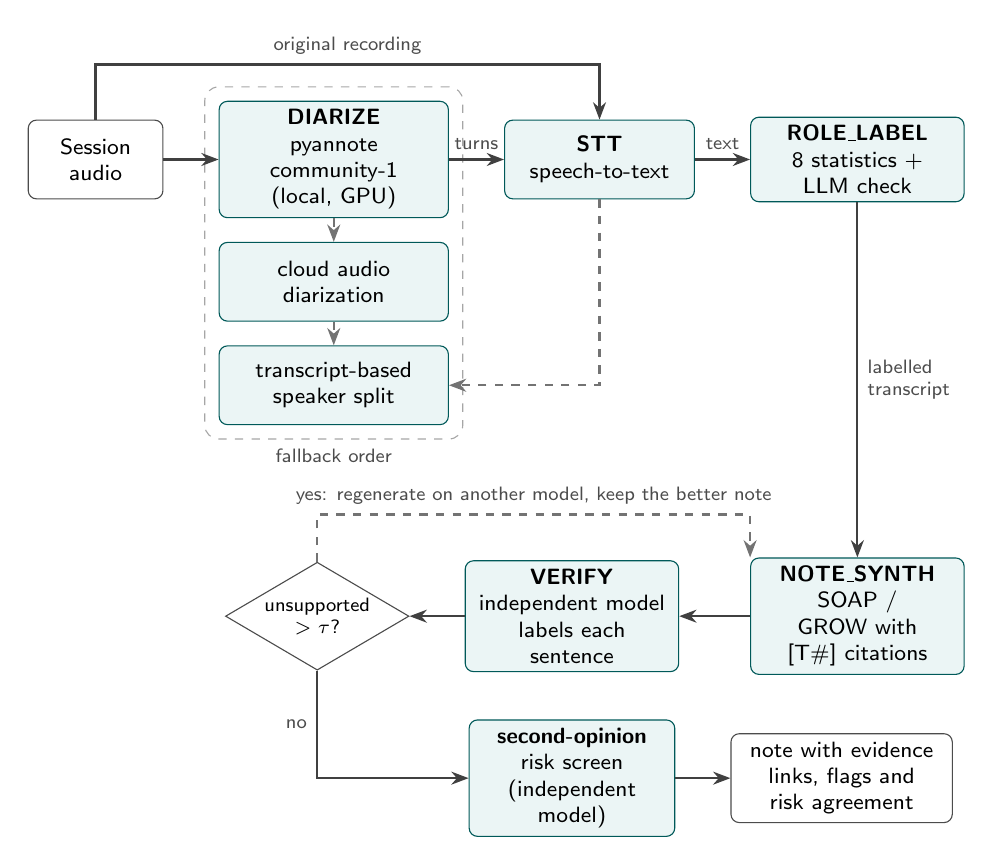
\begin{tikzpicture}[
  font=\sffamily\footnotesize,
  >={Stealth[length=2.2mm]},
  stage/.style={draw=black!70, rounded corners=3pt, fill=white, align=center, minimum height=10mm, inner sep=3pt, text width=#1},
  stage/.default=21mm,
  role/.style={draw=teal!70!black, rounded corners=3pt, fill=teal!8, align=center, minimum height=10mm, inner sep=3pt, text width=#1},
  role/.default=21mm,
  decision/.style={draw=black!70, diamond, aspect=1.7, fill=white, align=center, inner sep=1pt, font=\sffamily\scriptsize},
  flow/.style={->, thick, black!75},
  alt/.style={->, thick, dashed, black!55},
  lbl/.style={font=\sffamily\scriptsize, text=black!70},
  group/.style={draw=black!35, rounded corners=5pt, dashed, inner sep=5pt}
]
% ── row 1: original recording → speaker separation and STT → roles (no denoising) ──
\node[stage=15mm] (audio) {Session\\audio};
\node[role=27mm, right=7mm of audio] (sb) {\textbf{DIARIZE}\\pyannote community-1\\(local, GPU)};
\node[role=27mm, below=3mm of sb] (cloud) {cloud audio\\diarization};
\node[role=27mm, below=3mm of cloud] (text) {transcript-based\\speaker split};
\node[role=22mm, right=7mm of sb] (stt) {\textbf{STT}\\speech-to-text};
\node[role=25mm, right=7mm of stt] (roles) {\textbf{ROLE\_LABEL}\\8 statistics +\\LLM check};
\node[group, fit=(sb)(cloud)(text), label={[lbl]below:fallback order}] (diargrp) {};

\draw[flow] (audio) -- (sb);
\draw[flow] (audio.north) |- ++(0,7mm) -| node[lbl, pos=0.25, above] {original recording} (stt.north);
\draw[alt] (sb) -- (cloud);
\draw[alt] (cloud) -- (text);
\draw[flow] (sb) -- node[lbl, above] {turns} (stt);
\draw[flow] (stt) -- node[lbl, above] {text} (roles);
\draw[alt] (stt.south) |- (text.east);

% ── row 2: note writing, verification, gate, risk ──
\node[role=25mm] (writer) at (roles |- 0,-58mm) {\textbf{NOTE\_SYNTH}\\SOAP / GROW with\\{[}T\#{]} citations};
\node[role=25mm, left=9mm of writer] (verify) {\textbf{VERIFY}\\independent model\\labels each sentence};
\node[decision, left=7mm of verify] (gate) {unsupported\\$>\tau$?};
\node[role=24mm, below=6mm of verify] (risk) {\textbf{second-opinion}\\risk screen\\(independent model)};
\node[stage=26mm, right=7mm of risk] (out) {note with evidence\\links, flags and\\risk agreement};

\draw[flow] (roles) -- node[lbl, right, align=left] {labelled\\transcript} (writer);
\draw[flow] (writer) -- (verify);
\draw[flow] (verify) -- (gate);
\draw[alt] (gate.north) -- ++(0,6mm) -| node[lbl, pos=0.25, above] {yes: regenerate on another model, keep the better note} (writer.north west);
\draw[flow] (gate.south) |- node[lbl, pos=0.25, left] {no} (risk.west);
\draw[flow] (risk) -- (out);
\end{tikzpicture}
\caption{EchoScribe pipeline. Shaded boxes are processing roles, each served by a combo of the embedded router (Section~\ref{sec:router}). Speaker separation falls back from local pyannote to cloud audio diarization to a transcript-based split (dashed). The note writer cites transcript turns; an independent model (another vendor, else another model) verifies each sentence, and notes over the unsupported threshold $\tau$ are regenerated on another model. A second model screens independently for risk.}
\label{fig:pipeline}
\end{figure*}

Fig.~\ref{fig:pipeline} shows the pipeline. A browser client records or uploads audio; an Express.js server coordinates every model call; Supabase stores records under per-user row-level security, with therapy and mentoring records separated by a mode column that every query must state. Five roles call language or speech models: \role{STT}, \role{DIARIZE}, \role{ROLE\_LABEL}, \role{NOTE\_SYNTH} and \role{VERIFY}.

\subsection{Embedded multi-provider router}\label{sec:router}
Each role is served by a \emph{combo}: an ordered list of targets $\langle$vendor, model, keys$\rangle$ and a routing strategy. Vendors are thin adapters; Gemini~\cite{gemini2023}, Groq-hosted gpt-oss-120b~\cite{openai2025gptoss} and Whisper~\cite{radford2023whisper}, Deepgram and a local pyannote service ship as adapters, and OpenAI-compatible APIs are added by configuration. Several keys for one model form a pool whose keys take turns. The strategy orders targets per request: \emph{priority} (declared order; the next target is used only when every key of the current one is cooling down or retired, or the model itself fails), \emph{round-robin}, \emph{random}, \emph{strict-random}, \emph{least-used}, and \emph{lkgp} (the last target that succeeded goes first).

Failures are classified. A key that fails authentication is retired; a rate-limited or failing key enters an exponential cooldown of $5\cdot 2^{k-1}$~s (capped at 5~min) after its $k$-th consecutive failure, reset on success; a vendor with 15 failures within 30~min is skipped for 10~min (2 in 5~min for the local service); an HTTP~400 is treated as specific to the request and moves on without cooling the key. These mechanisms and constants are adapted from OmniRoute~\cite{omniroute2026}. When every target fails the API returns HTTP~503 with the attempts. Keys stay in the user's browser unless the user syncs one, which is then stored encrypted.

\subsection{Speech processing and role resolution}\label{sec:speech}
The recording is not denoised: SepFormer enhancement, our first design, raised word error rates (Section~\ref{sec:eval}), as reported for other front ends~\cite{iwamoto2022}. \role{DIARIZE} runs pyannote community-1~\cite{bredin2023pyannote,plaquet2023powerset} locally on the original 16~kHz recording, on a GPU when present, with two speakers and non-overlapping turns; it falls back to cloud audio diarization, then to splitting the transcript with a language model. \role{STT} transcribes the original recording; when the recogniser returns word timestamps (Whisper, Deepgram), each word goes to the turn that contains it~\cite{bain2023whisperx}, otherwise text is spread over turns by duration. A denoised copy (FFmpeg) is made only for listening again.

Roles are resolved without voice enrolment. For each speaker the system computes eight statistics: speaking time, word count and mean turn length, questions, professional vocabulary, guiding phrases, personal and emotional phrases, number of turns, and who spoke first. \role{ROLE\_LABEL} receives the transcript with these statistics and must assign exactly one professional and one client; invalid answers move to the next target, and a deterministic default is used only if every target fails.

\subsection{Evidence-linked notes, verification and repair}\label{sec:grounding}
The labelled transcript is numbered into turns $T_1\dots T_n$. \role{NOTE\_SYNTH} must end every sentence of the note sections, and of the risk notes, with the turns that support it (``\dots poor sleep for two weeks [T4, T6]''), write one fact per sentence, and write ``Not discussed'' rather than an uncited sentence. Citations are parsed into per-sentence evidence and removed from the displayed text. \role{VERIFY} receives each sentence with only its cited turns and labels it \emph{supported}, \emph{partial} (adds a detail the turns lack) or \emph{unsupported}. Verifiers are ordered another vendor first, then another model of the writer's vendor, and never the writer's own model. If the unsupported fraction exceeds $\tau=0.2$, the note is regenerated with the writer's model moved to the end of the combo, re-verified, and the draft with fewer unsupported sentences is kept.

Two further steps work at sentence level. \emph{Repair}: each flagged sentence goes back to a writer model with the transcript and the verifier's reason to be rewritten with citations, or removed if the transcript does not support it; rewrites are verified again. \emph{Two-judge agreement}: a flag stands only if a second judge, chosen to differ from the first and from the writer, also flags it. \ifrecheck These steps are evaluated in Section~\ref{sec:eval}.\else They are implemented in the released code but not evaluated in this paper.\fi The interface shows each sentence's evidence on hover and marks partial and unsupported sentences (Fig.~\ref{fig:ui}).

\begin{figure}[t]
\centering
{\footnotesize\textbf{(a)}}\\[1pt]
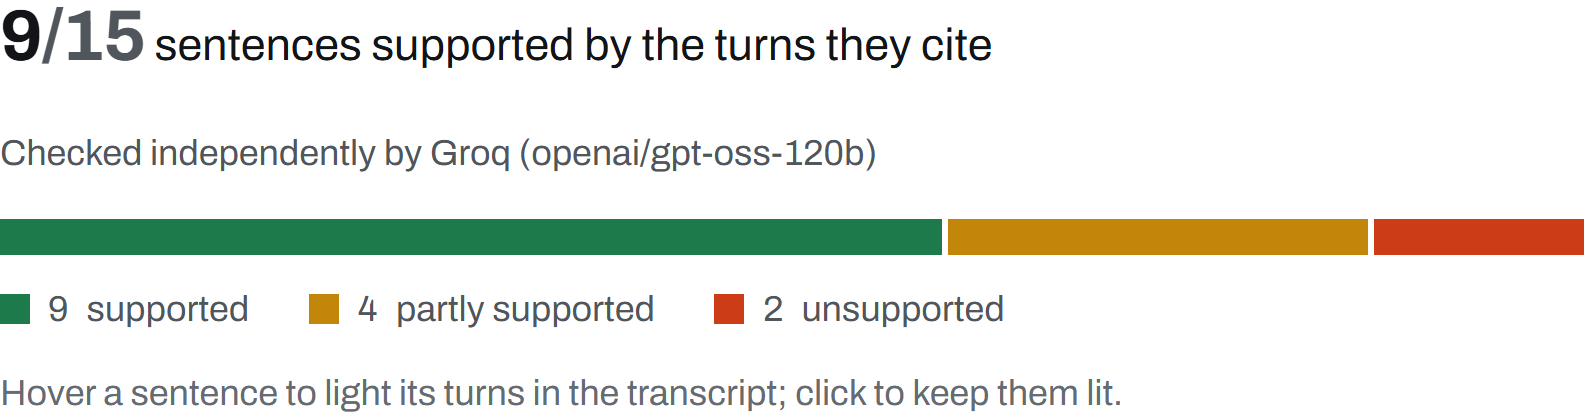
\includegraphics[width=0.78\columnwidth]{figures/ui_bar.png}\\[3pt]
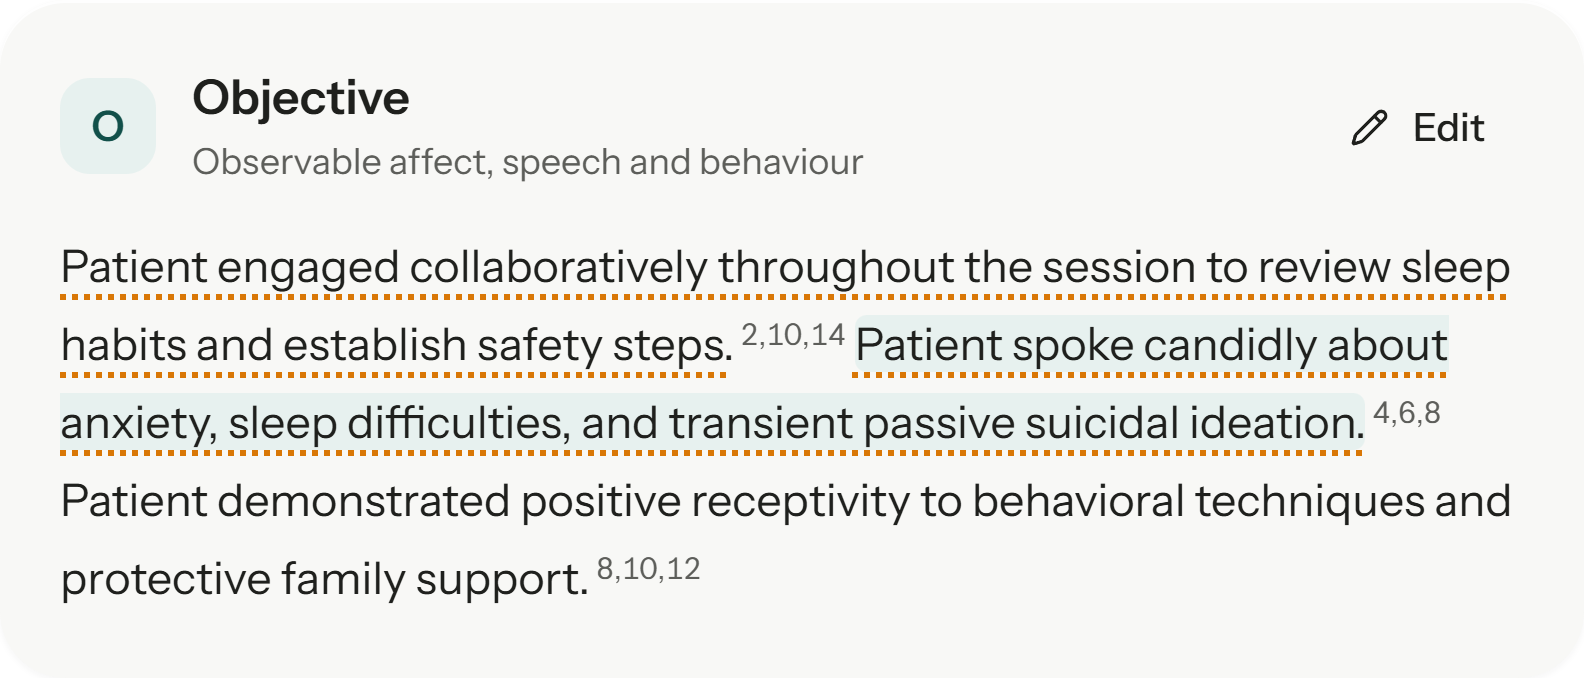
\includegraphics[width=0.78\columnwidth]{figures/ui_objective.png}\\[4pt]
{\footnotesize\textbf{(b)}}\\[1pt]
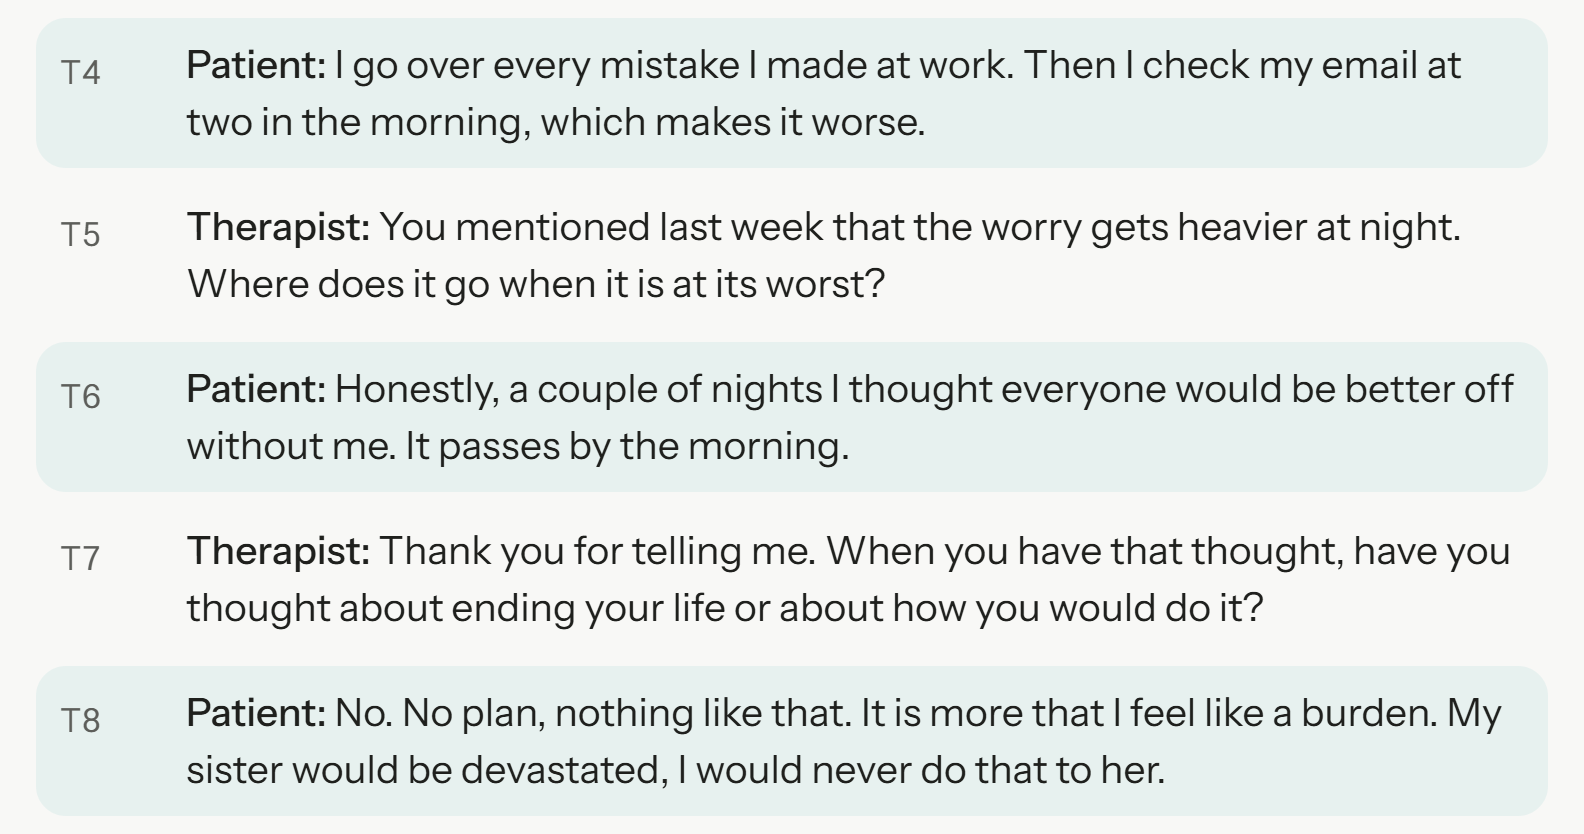
\includegraphics[width=0.78\columnwidth]{figures/ui_transcript.png}
\caption{EchoScribe's session summary for a scripted example session (invented transcript; real pipeline output). (a)~The verification bar counts sentences the independent verifier (here gpt-oss-120b, checking a Gemini-written note) judged supported, partly supported or unsupported; in the Objective section, dotted underlines mark partly supported sentences and superscripts give cited turns. (b)~Hovering the second Objective sentence highlights the turns it cites (T4, T6, T8) in the transcript.}
\label{fig:ui}
\end{figure}

\subsection{Risk screen with a second opinion}
In therapy mode the writer also screens for suicidal ideation and self-harm; in mentoring mode, for burnout and severe distress. A second model, chosen like the verifier, repeats the screen independently and cites its evidence turns. The flag is raised if either model raises it, favouring sensitivity, and disagreement is shown as ``models disagree --- review the transcript''. The screen is a model judgement, not a validated instrument such as the C-SSRS or PHQ-9~\cite{posner2011cssrs,kroenke2001phq9}, and the interface states that the clinician remains responsible for risk assessment.

\section{Evaluation}\label{sec:eval}
Every number below is generated from result files by scripts in the public repository (\texttt{eval/}); only free-tier model access was used.

\subsection{Setup}
\textbf{Data.} Notes are evaluated on the 40 test dialogues of ACI-Bench (test1, CC~BY~4.0)~\cite{yim2023aci}, whose doctor--patient visits have reference notes, and, without reference notes, on 40 high-quality motivational-interviewing dialogues of AnnoMI~\cite{wu2022annomi} drawn with a fixed seed over 32 topics. Real conversational speech comes from PriMock57~\cite{korfiatis2022primock57}: \ResPmN\ mock primary-care consultations (\ResPmHours~h) acted by clinicians and employees, with manual transcripts (CC~BY~4.0). Controlled noise tests use 12 simulated two-person conversations built from LibriSpeech test-clean~\cite{panayotov2015librispeech} (ten alternating utterances, 0.3--0.9~s gaps, exact reference turns), clean and with babble plus pink noise at 5~dB and 0~dB SNR.
\textbf{Models and metrics.} Gemini models~\cite{gemini2023} are used in rotation across three keys; gpt-oss-120b~\cite{openai2025gptoss} and Whisper large-v3~\cite{radford2023whisper} are served by Groq. We report ROUGE~\cite{lin2004rouge} and BERTScore~\cite{zhang2020bertscore} against reference notes, WER after text normalisation, DER with a 0.25~s collar~\cite{bredin2017metrics}, and cpWER, the speaker-attributed WER of CHiME-6~\cite{watanabe2020chime6}. Intervals are Wilson 95\%; differences are tested with a paired bootstrap (10{,}000 resamples).

\subsection{Router under injected faults}
We drive the router's own code with simulated vendors on a virtual clock: one hour of Poisson traffic at 10 requests/min against a preferred vendor (two keys), a fallback vendor (two keys) and a second fallback, in three scenarios: a per-key quota below the offered load, a 15-minute outage of the preferred vendor, and a \emph{mixed} case with a revoked key, a quota and a fallback that times out 20\% of the time. We compare walking the chain with no memory, the fixed 60~s suspension of our earlier design, and three strategies (5 seeds, Table~\ref{tab:router}).

\begin{table}[t]
\caption{Router in the mixed-fault scenario (mean of 5 seeds): success rate, failed provider calls per request, 95th-percentile latency.}
\label{tab:router}
\centering\footnotesize
\setlength{\tabcolsep}{6pt}
\begin{tabular}{@{}lrrr@{}}
\toprule
Policy & Success & Failed calls/req. & p95 (s) \\
\midrule
No memory   & \ResRouterMixedNomemorySuccess & \ResRouterMixedNomemoryFailed & \ResRouterMixedNomemoryPninetyfive \\
Fixed 60 s  & \ResRouterMixedFixedSuccess & \ResRouterMixedFixedFailed & \ResRouterMixedFixedPninetyfive \\
Priority    & \ResRouterMixedPrioritySuccess & \ResRouterMixedPriorityFailed & \ResRouterMixedPriorityPninetyfive \\
Round-robin & \ResRouterMixedRoundrobinSuccess & \ResRouterMixedRoundrobinFailed & \ResRouterMixedRoundrobinPninetyfive \\
LKGP        & \ResRouterMixedLkgpSuccess & \ResRouterMixedLkgpFailed & \ResRouterMixedLkgpPninetyfive \\
\bottomrule
\end{tabular}
\end{table}

Where a healthy fallback exists no policy changes success much, so differences lie in wasted calls and latency. Last-known-good stops returning to a vendor that keeps timing out and cuts mixed-scenario p95 latency from \ResRouterMixedPriorityPninetyfive~s to \ResRouterMixedLkgpPninetyfive~s (difference \ResSigRouterCi, \ResSigRouterP, faster in all 5 seeds). Under a per-key quota, round-robin and LKGP wasted \ResRouterQuotaRoundrobinFailed\ and \ResRouterQuotaLkgpFailed\ failed calls per request against \ResRouterQuotaPriorityFailed\ for priority; exponential cooldown alone is not uniformly better, because its 5~s first step re-probes an exhausted key. Priority keeps the preferred model at the cost of probing; LKGP minimises latency but can stay on a fallback after the preferred model recovers.

\subsection{Evidence-linked notes and independent verification}
\textbf{Does citing evidence reduce unsupported content?} With the same Gemini writer and prompt apart from the citation rule, we wrote a single-pass SOAP note and an evidence-linked note for each of the \ResBaseN\ dialogues, shuffled the sentences of both, and had a judge from another vendor (gpt-oss-120b) label each against the \emph{full} transcript without knowing its source (Table~\ref{tab:notes}). Evidence-linked notes had fewer unsupported sentences (\ResBaseLinkedUnsupported\ against \ResBaseSingleUnsupported, non-overlapping intervals), fewer notes with any unsupported sentence (\ResBaseLinkedNotesUnsupported\ against \ResBaseSingleNotesUnsupported), and no lower ROUGE or BERTScore.

\begin{table}[t]
\caption{Notes on ACI-Bench test1. Top: single-pass vs evidence-linked notes from the same writer, every sentence judged blind against the full transcript by another vendor. Bottom: planted errors caught by the verifier, and false alarms on unchanged sentences.}
\label{tab:notes}
\centering\footnotesize
\setlength{\tabcolsep}{4pt}
\begin{tabular}{@{}lrr@{}}
\toprule
 & Single-pass & Evidence-linked \\
\midrule
Sentences per note & \ResBaseSingleSentences & \ResBaseLinkedSentences \\
Supported (95\% CI) & \ResBaseSingleSupported\ (\ResBaseSingleSupportedCi) & \ResBaseLinkedSupported\ (\ResBaseLinkedSupportedCi) \\
Partly supported & \ResBaseSinglePartial & \ResBaseLinkedPartial \\
Unsupported (95\% CI) & \ResBaseSingleUnsupported\ (\ResBaseSingleUnsupportedCi) & \ResBaseLinkedUnsupported\ (\ResBaseLinkedUnsupportedCi) \\
Notes with an unsupported sentence & \ResBaseSingleNotesUnsupported & \ResBaseLinkedNotesUnsupported \\
ROUGE-1 / 2 / L & \ResBaseSingleRougeOne\,/\,\ResBaseSingleRougeTwo\,/\,\ResBaseSingleRougeL & \ResBaseLinkedRougeOne\,/\,\ResBaseLinkedRougeTwo\,/\,\ResBaseLinkedRougeL \\
BERTScore F1 & \ResBaseSingleBert & \ResBaseLinkedBert \\
\midrule
 & Gemini-written & gpt-oss-written \\
\midrule
Changed number caught & \ResInjGemNum & \ResInjGroqNum \\
Flipped negation caught & \ResInjGemNeg & \ResInjGroqNeg \\
Borrowed sentence caught & \ResInjGemFab & \ResInjGroqFab \\
False alarms on unchanged & \ResInjGemFa & \ResInjGroqFa \\
\bottomrule
\end{tabular}
\end{table}

\textbf{Two writers and the cascade.} Each of two writers also produced evidence-linked notes judged against only their cited turns, the stricter test the interface uses. Citation coverage was \ResGroundGemCited\ (Gemini) and \ResGroundGroqCited\ (gpt-oss-120b), with \ResGroundGemSupported\ and \ResGroundGroqSupported\ of sentences supported and \ResGroundGemUnsupported\ and \ResGroundGroqUnsupported\ unsupported. Where the Groq daily cap was reached, verification of Gemini-written notes was cross-model, not cross-vendor (\ResVerGemCrossVendor\ notes cross-vendor, \ResVerGemCrossModel\ cross-model). With $\tau=0.2$, \ResCascadeEscalated\ of \ResCascadeNotes\ Gemini-first notes would have been regenerated.

\textbf{Does the verifier catch errors?} We planted three kinds of error into sentences the verifier had accepted (a changed number, a flipped negation, and a sentence borrowed from another dialogue's note with its citations) and kept other accepted sentences as controls. Across \ResInjPlantedN\ planted errors the verifier flagged \ResInjRecallPct\ as partial or unsupported, with \ResInjFaPct\ false alarms on \ResInjControlN\ unchanged sentences (Table~\ref{tab:notes}, bottom); controls had already been accepted, so this measures consistency, not precision on fresh sentences.

\textbf{Counselling dialogues.} On AnnoMI, evidence-linked notes (without sentence repair) for \ResAnnoNotesN\ dialogues had \ResAnnoSentences\ sentences, \ResAnnoCited\ cited, of which \ResAnnoSupported\ were judged supported, \ResAnnoPartial\ partly and \ResAnnoUnsupported\ unsupported. These judgements are not vendor-independent: \ResAnnoJudgeGeminiN\ of \ResAnnoNotesN\ notes were checked by a Gemini model other than the writer's, because the Groq quota was exhausted.

\ifrecheck
\textbf{Repair and a held-out judge.} Writing one fact per sentence, then repairing flagged sentences, changed the same \ResAblNotes\ ACI notes as follows. The pipeline's own judge rated \ResAblVerSupported\ of \ResAblSentences\ sentences supported as written and \ResAblRepSupported\ after repair (\ResAblRepairRewritten\ of \ResAblRepairFlagged\ flagged sentences rewritten, \ResAblRepairRemoved\ removed). That judge also chose the sentences to repair, so we re-judged the final sentences of \ResAblHeldNotes\ notes (\ResAblHeldSentences\ sentences) with a held-out judge, Groq gpt-oss-120b: \ResAblHeldSupported\ supported (\ResAblHeldSupportedCi), \ResAblHeldUnsupported\ unsupported, agreeing with the pipeline's labels on \ResAblHeldAgree. The held-out figure is our estimate. Overlap with the reference notes also rose (ROUGE-1/2/L \ResAblRougeOne/\ResAblRougeTwo/\ResAblRougeL, BERTScore \ResAblBert, against \ResBaseLinkedRougeOne/\ResBaseLinkedRougeTwo/\ResBaseLinkedRougeL\ and \ResBaseLinkedBert\ before these steps).
\fi

\subsection{Role identification}
With speaker labels replaced by random identifiers, the eight statistics alone named the clinician correctly in \ResRoleStatsCorrect\ of \ResRoleN\ ACI-Bench dialogues, the model alone in \ResRoleLlmCorrect, and their combination, as deployed, in \ResRoleCombinedCorrect\ (\ResRoleCombined). Only \ResRoleHardN\ ACI dialogues had the patient speaking more than the doctor. In AnnoMI counselling the client often talks more: statistics alone were right in \ResAnnoRoleStats\ of \ResAnnoRoleN\ dialogues, the model alone in \ResAnnoRoleLlm, and the combination in \ResAnnoRoleCombined; in the \ResAnnoRoleHardN\ dialogues where the client spoke more, the three methods were right in \ResAnnoRoleHardStats, \ResAnnoRoleHardLlm\ and \ResAnnoRoleHardCombined. On PriMock57 the deployed combination was right in \ResPmRoleCorrect\ of \ResPmRoleN\ consultations.

\subsection{Speech recognition and speaker attribution}
\begin{table}[t]
\caption{Speech results (\%). Top: simulated conversations (12 $\times$ 3 conditions): recognition with and without SepFormer denoising, and DER. Middle: speaker-attributed cpWER of each path; the first row is our first design, the bold row the current one. Bottom: PriMock57 mock consultations.}
\label{tab:speech}
\centering\footnotesize
\setlength{\tabcolsep}{3.5pt}
\begin{tabular}{@{}lrrr@{}}
\toprule
 & Clean & 5 dB & 0 dB \\
\midrule
WER Whisper, original / denoised & \ResAudioWerGroqRawClean\,/\,\ResAudioWerGroqEnhClean & \ResAudioWerGroqRawFive\,/\,\ResAudioWerGroqEnhFive & \ResAudioWerGroqRawZero\,/\,\ResAudioWerGroqEnhZero \\
WER Gemini, original / denoised & \ResAudioWerGemRawClean\,/\,\ResAudioWerGemEnhClean & \ResAudioWerGemRawFive\,/\,\ResAudioWerGemEnhFive & \ResAudioWerGemRawZero\,/\,\ResAudioWerGemEnhZero \\
DER pyannote / SpeechBrain & \ResAudioDerPyaClean\,/\,\ResAudioDerSbRawClean & \ResAudioDerPyaFive\,/\,\ResAudioDerSbRawFive & \ResAudioDerPyaZero\,/\,\ResAudioDerSbRawZero \\
\midrule
SepFormer + SpeechBrain + Gemini & \ResAudioCpSbEnhClean & \ResAudioCpSbEnhFive & \ResAudioCpSbEnhZero \\
pyannote + Whisper, by duration & \ResAudioCpPyaPropClean & \ResAudioCpPyaPropFive & \ResAudioCpPyaPropZero \\
\textbf{pyannote + Whisper, by word time} & \textbf{\ResAudioCpPyaWordsClean} & \textbf{\ResAudioCpPyaWordsFive} & \textbf{\ResAudioCpPyaWordsZero} \\
SpeechBrain + Whisper, by word time & \ResAudioCpSbWordsClean & \ResAudioCpSbWordsFive & \ResAudioCpSbWordsZero \\
Cloud audio diarization (Gemini) & \ResAudioCpGemAudioClean & \ResAudioCpGemAudioFive & \ResAudioCpGemAudioZero \\
\midrule
\multicolumn{4}{@{}l}{PriMock57, \ResPmN\ consultations, \ResPmHours~h (pyannote + Whisper)} \\
DER / WER & \multicolumn{3}{c}{\ResPmDer\,/\,\ResPmWer} \\
cpWER by word time / by duration & \multicolumn{3}{c}{\ResPmCpWords\,/\,\ResPmCpDuration} \\
\bottomrule
\end{tabular}
\end{table}

Table~\ref{tab:speech} reports the speech results. Denoising before recognition, as in our first design, raised word error rates under noise for both recognisers (Whisper at 0~dB from \ResAudioWerGroqRawZero\% to \ResAudioWerGroqEnhZero\%; \ResSigWerWhisperZeroP\ and \ResSigWerGeminiZeroP\ for Whisper and Gemini), so the deployed pipeline transcribes the original recording. pyannote separated speakers with \ResAudioDerPyaClean\% DER on clean audio against \ResAudioDerSbRawClean\% for SpeechBrain clustering (\ResSigDerPyaCleanP; at 5~dB \ResSigDerPyaFiveP). Speaker attribution depends as much on placing words as on finding turns: spreading the transcript over pyannote's turns by duration gave \ResAudioCpPyaPropClean\% cpWER on clean audio, and assigning each word to the turn containing its Whisper timestamp gave \ResAudioCpPyaWordsClean\% (\ResSigWordsDurCleanP\ in all three conditions). Against cloud audio diarization the local pipeline attributed better on clean audio (\ResSigWordsCloudCleanP) and at 5~dB (\ResAudioCpPyaWordsFive\% against \ResAudioCpGemAudioFive\%, \ResSigWordsCloudFiveP). At 0~dB pyannote's DER rises to \ResAudioDerPyaZero\% (\ResSigDerPyaZeroP\ against SpeechBrain), and SpeechBrain clustering with word timestamps attributes slightly better (\ResAudioCpSbWordsZero\% against \ResAudioCpPyaWordsZero\%); the difference from cloud diarization at 0~dB is not significant (\ResSigWordsCloudZeroP). On real mock consultations the same pipeline reached \ResPmDer\ DER and \ResPmWer\ WER, with \ResPmCpWords\ speaker-attributed error against \ResPmCpDuration\ when words were spread by duration.

Per minute of audio, pyannote took \ResLatPyaGpu~s on a laptop GPU (RTX~4050) and \ResLatPyaCpu~s on its CPU, against \ResLatSbEnh~s for the first design's SepFormer enhancement with SpeechBrain diarization; Whisper on Groq took \ResLatSttGroq~s and Gemini speech-to-text \ResLatSttGem~s.

\ifmentoring
\subsection{GROW notes on mentoring sessions}
We ran \ResMenSessions\ \MentoringAudioDesc\ (\ResMenMinutes~min in total, \ResMenMentees\ mentee personas) through the deployed pipeline end to end. pyannote found two speakers in \ResMenTwoSpk\ sessions and role resolution assigned one mentor and one mentee in \ResMenRoles; \ResMenGrowAll\ notes filled all four GROW sections. Notes had \ResMenPerNote\ sentences on average, \ResMenCited\ cited; the pipeline's judge rated \ResMenSupported\ supported, \ResMenPartial\ partly and \ResMenUnsupported\ unsupported, and repair rewrote \ResMenRepairRewritten\ of \ResMenRepairFlagged\ flagged sentences and removed \ResMenRepairRemoved. Processing took \ResMenRtf~s per minute of audio. These sessions come from \ResMenMentees\ personas and are not independent samples, the judge is not held out, and no human rating of GROW content is reported, so the figures show feasibility, not accuracy.
\fi

\section{Discussion and Limitations}
\textbf{What the results support.} Citation-constrained writing halved unsupported content against a single-pass note without lowering overlap with reference notes, and an independent verifier caught most planted factual errors, so sentence-level flags give a reviewer a concrete place to look instead of an unexplained confidence score~\cite{guo2017calibration}. Resilience in the router comes from remembering failures. Placing words by timestamp, not turn duration, accounts for most of the gain in speaker attribution on simulated and acted speech, and role identification without enrolment was accurate on medical and counselling dialogue.

\textbf{Deployment.} EchoScribe runs on the clinician's machine; only the configured model vendors receive audio or text, an institution can restrict processing to vendors its governance policy approves, and long recordings are compacted before reaching a cloud model.

\textbf{Limitations.} (i) ACI-Bench and PriMock57 are medical, and AnnoMI has no reference notes; no public corpus of counselling or mentoring sessions with reference notes exists\ifmentoring, and the mentoring sessions we ran are few and not independent\else, so GROW notes were not evaluated\fi. (ii) Support labels come from a model; the planted-error test bounds how often it misses errors of three kinds, but subtler omissions and misattributions need human review~\cite{asgari2025}, and where a quota forced a judge from the writer's vendor the check was not vendor-independent. (iii) Simulated speech is read without overlap, and PriMock57 is acted speech; overlapping, emotional clinical speech will be harder, and at 0~dB our attribution is not better than cloud diarization. (iv) Results depend on specific model versions that vendors retire; we log the serving model of every request. (v) The risk screen has not been validated against clinician labels. Blinded rating kits for notes and verifier agreement are released with the code. \textbf{Ethics:} no human-subject data were used; all experiments use public datasets and scripted or synthetic material, and free-tier model vendors may use submitted text for training, so deployments with real sessions should use institutionally approved vendors or local models.

\section{Conclusion}
EchoScribe produces SOAP and GROW notes from recorded two-person sessions in which every sentence points to the turns that support it and is checked by a model other than its writer, with regeneration of failing notes, a two-model risk screen that surfaces disagreement, and an embedded router that keeps every processing role available through quota exhaustion and outages. Citing evidence halved unsupported content against a single-pass note from the same writer; assigning words to speakers by timestamp cut speaker-attributed error from \ResPmCpDuration\ to \ResPmCpWords\ on mock consultations; and role identification needed no enrolment. The code, evaluation scripts and rating kits are available at \url{https://github.com/Aravind-Krishnan-S/ECHOSCRIBE}.

\section*{Acknowledgment}
The authors thank the faculty of the Department of Artificial Intelligence and Data Science at Jyothi Engineering College for their guidance, and the pyannote, SpeechBrain, ACI-Bench, AnnoMI, PriMock57, LibriSpeech and OmniRoute communities for openly licensed models, data and code. Claude (Anthropic) was used to draft and revise the manuscript text and LaTeX, and to write parts of the software and evaluation code; the authors directed, verified and take responsibility for all content.

\bibliographystyle{IEEEtran}
\bibliography{refs}

\end{document}
